\chapter{Optimizing the synthesis of monodisperse colloidal spheres}
\label{ch:synthesis}

\section{Introduction}

The earliest reference to emulsion polymerization dates back to
1909 \cite{bayer1909,finch03} to a patent awarded to Felix Hoffmann and
co-workers at Farbenfabriken Bayer for their pioneering work in manufacturing
synthetic latex.
Techniques for polymerizing emulsions have progressed  over the ensuing century
through intuitive leaps guided by fundamental principles of chemistry
and physics.  Controlling the size, monodispersity, and composition of
colloidal spheres is crucial for many applications including micrometer-scale
self-assembly \cite{pusey87,sacanna11}. Most often, the influences of particular chemical
or physical conditions on the properties of synthetic colloids only can be gauged once
synthesis is complete; these assays typically require multiple orthogonal measurement
techniques.
Scanning electron microscopy, for example, is used to measure solid particles'
size distribution and surface texture. Mercury porosimetry gauges their
porosity. Techniques such as refractometry probe their optical properties.
Amassing a representative set of characterization results takes considerable
time and requires
expertise in multiple techniques. Furthermore, sample preparation for any one
of these technique can change their \emph{in situ} properties.
Correlations among particle properties are especially difficult to measure.

Holographic particle characterization can streamline this analysis by providing
particle-resolved assays of samples' size distributions and compositions rapidly and with
minimal sample preparation. Holographic characterization works equally
well for droplets and solid particles. It naturally accommodates heterogeneous
samples and reveals correlations between size and composition. Extensions to the technique
provide particle-resolved morphology measurements from the same underlying data.
All of this information about a sample's properties can be acquired with a
single measurement in under a half an hour, which
expedites systematic assays and can be fast enough to provide feedback
for process control.

%Holographic assays provide information that is useful for designing synthetic
%pathways and can help to detect and diagnose deficiencies. These measurements
%can proceed rapidly enough, moreover, to provide real-time feedback during
%synthesis. We illustrate these capacities by analyzing the synthesis of a
%particularly interest colloidal suspension.

In this chapter, we use holographic particle characterization
to explore the roles of stoichiometry, initiator choice, and
agitation conditions in the synthesis of monodisperse spheres of
3-(trimethoxysilyl)propyl methacrylate (TPM) \cite{vanderwel17},
a model system with increasingly widespread applications
in soft-matter research \cite{sacanna11,liu16,vanderwel18}.
We employ holographic characterization
in tandem with conventional particle characterization
techniques to identify factors that influence size selection, polydispersity
and composition.
These orthogonal measurements also serve to validate the results observed
holographically.
This study extends the work of van der Wel \emph{et} \emph{al.} \cite{vanderwel17}, which
uses conventional characterization techniques to systematically
characterize the emulsion polymerization protocol for TPM spheres.

\section{Synthesizing TPM spheres}

Since their introduction in 2010 \cite{sacanna10}, TPM spheres have been used as
model systems of soft matter research to
study self-assembly \cite{sacanna13} and active matter \cite{palacci13}.
They are particularly attractive for optical studies because they can be
simultaneously density matched and index matched to their surrounding
medium \cite{liu16}.
A comparatively straightforward synthesis readily produces monodisperse spheres
with sizes selected reproducibly in the range of a few hundred nanometers to a
few micrometers \cite{liu16}.
Unlike the better-known syntheses of polystyrene \cite{goodwin1974} and
silica \cite{stober68},
emulsion polymerization of TPM requires no specialized equipment or
inert environment.

\subsection{Emulsion polymerization}
\label{ssec:polymerization}

Our procedure for synthesizing TPM spheres is described in section
\ref{ssec:synthesizing_tpm}, with the
exception of initiator choice. We reiterate the synthesis protocol
here to underscore the conditions we varied and to motivate the choices
made for the
\num{32} samples of droplets and polymerized spheres that we analyzed.
A detailed account of the polymer chemistry underlying this
protocol is provided in Ref.~\cite{vanderwel17}.

The protocols chosen for this study illuminate the influence of stir rate, pH,
emulsion stoichiometry, and radical initiator choice on the size and refractive index
of the synthesized particles. While this list is not exhaustive,
it illustrates choices made in optimizing synthesis protocols and the role
that holographic characterization can play in making successful choices.

The synthesis begins with the formation of an emulsion of monodisperse TPM droplets.
Monomeric TPM, ((3-(trimethoxysilyl)propyl methacrylate, \SI{98}{\percent}, Sigma Aldrich)
is insoluble in water. When it is added to the basic environment
of ammonium chloride (\SI{29}{\percent}) in water (pH $>$ \num{9}),
the monomers undergo hydrolysis and become soluble. 
Hydrolyzed monomers then form insoluble 
oligomers that condense homogeneously into monodisperse droplets.
These nuclei continue to grow in a well-mixed environment as more oligomers form.
The droplets stop growing once the free hydrolyzed monomer is depleted and
oligomerization ends. The length of the growth period is empirically determined
through trial and error. Once growth is complete, the droplets are still fluid
but are largely stable against coarsening. They can be polymerized into
solid spheres by heating the emulsion to \SI{80}{\degreeCelsius}
and adding a heat activated free radical initiator.

The process of nucleation and growth of oligomerized TPM droplets can be
affected by changing chemical and physical conditions.
Dissociation of ammonium chloride in water leads to the production of ammonia
gas, which escapes the solution and reduces its pH.
To mitigate this effect, the emulsion is prepared in a closed vial.
%In preparing a battery of spheres for comparative studies,
In addition,
we use identical \SI{12}{\milli\liter} vials to produce \SI{5}{\milli\liter}
of colloidal suspension so that the volume of enclosed air, and therefore
the loss in pH, is reproducible. Identical stir bars are
used for all syntheses to ensure consistent flow properties.

\subsection{Holographic particle characterization}

We perform holographic characterization measurements with a Spheryx xSight,
a commercial holographic particle characterization system
that automates the methods described in the previous chapters.
The xSight draws a small sample of colloidal suspension through the
observation volume of a conventional microscope where it is illuminated
with a laser operating at a vacuum wavelength of \SI{532}{\nm}.
The instrument's analytical software processes particles' holograms automatically
and yields the size and refractive index for each observed colloidal sphere
in a fraction of the time we typically spend analyzing an experimental video.
Because we are particularly interested in collecting population statistics for the sizes
and refractive
indexes of our TPM samples, we utilize the xSight rather than our custom-built holographic
microscope.

The xSight cannot analyze colloidal dispersions with particle number densities exceeding
\SI{E6}{\milli\liter^{-1}} because crowding the observation volume with
particles creates overlapping holograms that are not reliably interpreted.
This limitation is discussed in section \ref{ssec:sample_prep}.
Because the emulsion polymerization process described in the previous section
produces samples with number densities of \SI{E10}{\milli\liter^{-1}},
we dilute each of our samples by a factor of \SI{E4}{} with
deionized water before analysis. This should not affect the particles'
properties because polymerized TPM is hydrophobic.

We analyze each sample by pipetting \SI{100}{\micro\liter} of the diluted
dispersion into an xCell microfluidic sample cell and loading the xCell into the xSight.
The xSight draws \SI{3}{\micro\liter} of the fluid through
the xCell's \SI{50}{\um} deep observation volume. A ten-minute measurement provides us with
characterization data for a few thousand colloidal spheres per sample.

\begin{figure}
    \centering
    \includegraphics[width=\columnwidth]{example_poiseuille_fit}
    \caption{The measured flow profile of particles streaming through the xCell.
      (a)  A diagram of the observed Poiseuille flow.\protect\footnotemark 
      (b) Scatter plot of average particle height and average velocities; each
      dot represents a single micrometer scatterer. Color denotes the density of
      observations. The fit to a parabolic flow profile is illustrated with a dashed
      blue line. (c) Scatter plot of data after filtering observations deviating
      from the parabolic profile.}
    \label{fig:flow_prof}
\end{figure}

\footnotetext{The focal plane is \SI{90}{\um} below the lower sample-xCell interface:
  a scale diagram would depict the focal plane inside the lower xCell wall.}

During a measurement, the sample flows between the stationary walls of the xCell
with a parabolic, Poiseuille profile.
The particles act as passive tracers of this flow.
The xSight uses holographic tracking data to map the local fluid velocity within
the channel \cite{cheong10a}, as shown in Fig.~\ref{fig:flow_prof}.
Each point in Fig.~\ref{fig:flow_prof}(a) represents the measured speed
and axial position, $v(z)$, for a single particle.
As illustrated in Fig.~\ref{fig:flow_prof}(a),
the particle's axial position is measured relative to the microscope's
focal plane. The solid curve in Fig.~\ref{fig:flow_prof}(b) is a fit to the
anticipated parabolic flow profile. Extrapolating this fit to $v(z)=0$ yields the
axial position of this channel's walls, assuming
no-slip boundary conditions. 
The majority of observations fall neatly onto the parabolic profile.
% Note that velocities should deviate by a small amount due to Brownian motion.
Some fits, however, deviate markedly. Presumably these data result from fitting
to false positive detections of overlapping holograms.
We suppress these erroneous features by rejecting data that deviate from
the parabolic profile by more than one median absolute deviation,
as depicted in Fig.~\ref{fig:flow_prof}(c). The remaining results are used
to characterize the sample.
% Why this degree of cutting?

\subsection{Orthogonal validation methods}

Holographic particle characterization is a comparatively new technique
and is not yet widely adopted. We therefore validate results from
holographic particle characterization with measurements from orthogonal
techniques.
Specifically, we use scanning electron microscopy to provide baseline estimates for the
particles' diameters and Abbe refractometry to measure their refractive indexes.

Each sample of polymerized spheres were imaged with a MERLIN (Carl Zeiss) field
emission scanning electron microscope (SEM).
Typical images are provided in Fig.~\ref{fig:sem_stir_rate}(a).
SEM images provide a visual check on the sample's uniformity
and can be used to estimate the colloidal spheres' diameter.
While a well calibrated scanning
electron microscope provides \num{1} to \SI{10}{\nm} spatial resolution, sample
preparation, particularly exposure to vacuum and sputter coating, can shrink or
even swell the sample \cite{yamada85,jung02}. Liquid TPM droplets
are not amendable to SEM analysis.

A common method for determining the refractive index of colloidal particles
involves index matching the particles to a solution with a known refractive index.
This procedure requires dispersing the particles in an index-matching solution
rather than their native medium and therefore necessitates
that the solution not affect the particle's properties, for
example by swelling.  Reference~\cite{vanderwel17} estimated the
refractive index of polymerized TPM colloids to lie between $\num{1.512}$ and $\num{1.513}$
by index matching to a solution of pyridine ($n = \SI{1.509}{}$) and \num{2}-ethylhexyl
\num{4}-methoxycinnamate ($n = \SI{1.545}{}$). We instead estimate the spheres'
refractive index by measuring the refractive index of the suspension as a function of
volume fraction in water. Extrapolating  to \SI{100}{\percent} volume fraction
yields an estimate for the spheres' refractive index \cite{alexander81} in their native medium.

\section{Influence of synthesis conditions}
\subsection{Effect of stir rate}
\label{ssec:stir}
Stirring the sample while the oligomers condense into droplets promotes homogeneous
nucleation by uniformly dispersing the hydrolyzed monomer and droplet nuclei.
Beyond simply mixing the sample, however, stirring creates shear forces that can
also alter droplets' size distribution.
The effect of stir rate on the resulting particle size is best assessed
experimentally.
We investigate the influence of stir rate by producing four sets of TPM emulsions
in four identical vials with identical stir bars. Each vial was filled with
\SI{15}{\micro\liter} of \SI{29}{\percent} ammonia followed by
\SI{200}{\micro\liter} of TPM monomer to \SI{5}{\milli\liter} of DI water.
The four samples were stirred for \SI{2}{\hour}
using magnetic stir plates set at \num{500}, \num{700}, \num{900}, and
\SI{1100}{\minute^{-1}}. 
The resulting droplets were polymerized by adding
\num{2},\num{2}'-azobis(\num{2}-methylpropionitrile) (AIBN, Sigma Aldrich)
as a radical initiator and %FIXME: Lot number of AIBN?
heating the sample to \SI{80}{\celsius} for \SI{2}{\hour}.
We prepared samples of unpolymerized droplets and samples of polymerized TPM spheres
at each of the four spin rates for a total of eight samples.

\begin{figure}
    \centering
    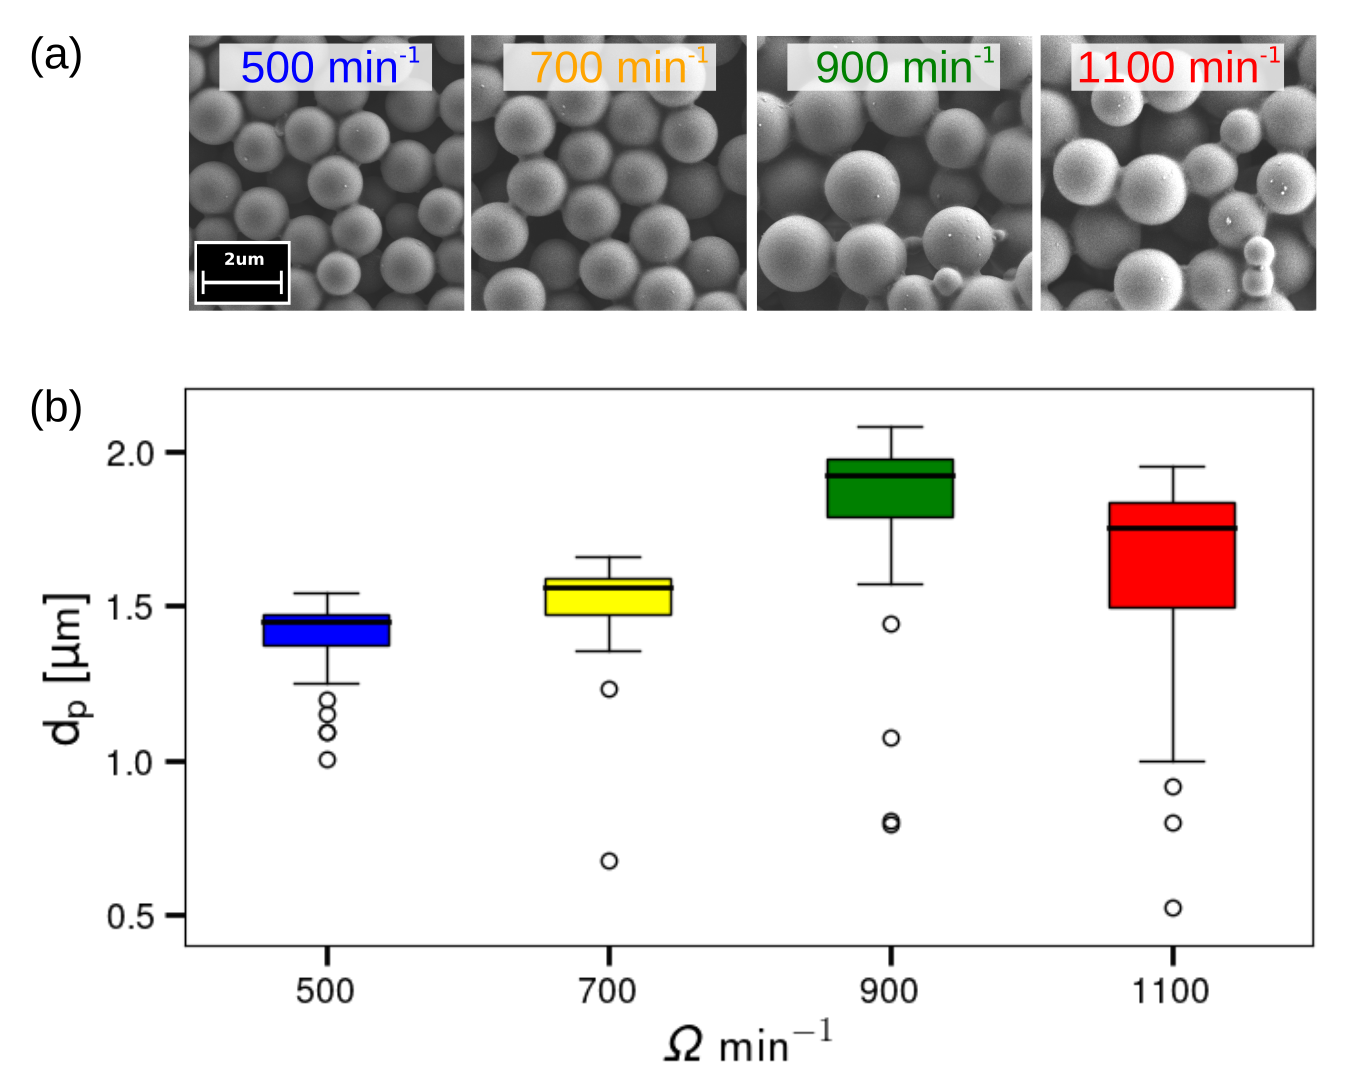
\includegraphics[width=0.8\columnwidth]{sem_stir_analysis}
    \caption{(a) Cropped and scaled SEM images of the polymerized TPM spheres whose
      samples were stirred at \num{500}, \num{700}, \num{900}, and \SI{1100}{\minute^{-1}}.
      (b)  Box and whisker plots summarize the diameters of colloidal spheres estimated from
      SEM digital images and are labeled with the same color convention as (a).
      Each rectangular box extends from the first quartile, $Q_1$, to
      the third quartile, $Q_3$, of the data; within each box a black line represents the median;
      the upper whisker extends to largest observed diameter less than $Q_3 + 1.5\, (Q_3 - Q_1)$;
      the lower whisker extends to the smallest observed diameter greater than $Q_1 - 1.5\, (Q_3 - Q_1)$;
      data beyond the whiskers are plotted as open circles. }
    \label{fig:sem_stir_rate}
\end{figure}

Each of the four samples of polymerized spheres were imaged with an SEM.
Figure~\ref{fig:sem_stir_rate}(a) shows cropped and scaled regions of interest
for each sample. The mean sphere diameter in a sample is estimated by analyzing
spheres' images using ImageJ \cite{mazzoli12}. % Find better citation?
The diameter of an individual sphere is obtained by
drawing a tight-fitting oval around its image;
the average of each oval's minor and major axes provides an estimate for the
associated sphere's diameter. Results of this manual survey are summarized in
Fig.~\ref{fig:sem_stir_rate}(b). The average 
diameters, $\avg{d_{\text{p}}}$, and their standard deviations, $\sigma_{d_{\text{p}}}$,
for each of the four stir rates are reported
in Table \ref{table:sem_data}.
Any trend in the mean diameter is obscured by the increase in polydispersity
with increasing stir rate. SEM analysis suggests that this may be
due to an increase in the population of undersized spheres with increasing
shear rate.

\begin{table}[b!]
\centering
\caption{Average size and standard deviation of TPM spheres measured from
SEM images for each of the four stir rates.}
\begin{tabular}{rlrrrr}
\hline
\hline
$\Omega$ & $[\si{\minute^{-1}}]$ & \num{500} & \num{700}& \num{900} & \num{1100} \\
\hline
$\avg{d_{\text{p}}}$ & $[\si{\um}]$ & 1.40 & 1.52 & 1.82 & 1.64 \\ 
$\sigma_{d_{\text{p}}}$ & $[\si{\um}]$ & 0.12 & 0.13 & 0.28 & 0.32 \\ \hline \hline
\end{tabular}
\label{table:sem_data}
\end{table}

Two similarly prepared samples of TPM spheres were used to estimate the refractive
index, $n_p$, of the colloidal spheres.
Each sample was diluted to \num{5} different volume fractions to provide a total of
\num{12} different suspensions, including the two stock samples.
The refractive index of each
suspension was measured with an Abbe refractometer;
the results are summarized in Fig.~\ref{fig:abbe}.
By assuming a linear relationship between volume fraction and suspension refractive
index, we estimate the refractive index of TPM colloidal spheres to be $n_{\text{p}} = \SI{1.506}{}$ with \SI{95}{\percent} confidence that it lies in the range $1.499 \le n_{\text{p}} \le 1.513$.

\begin{figure}
    \centering
    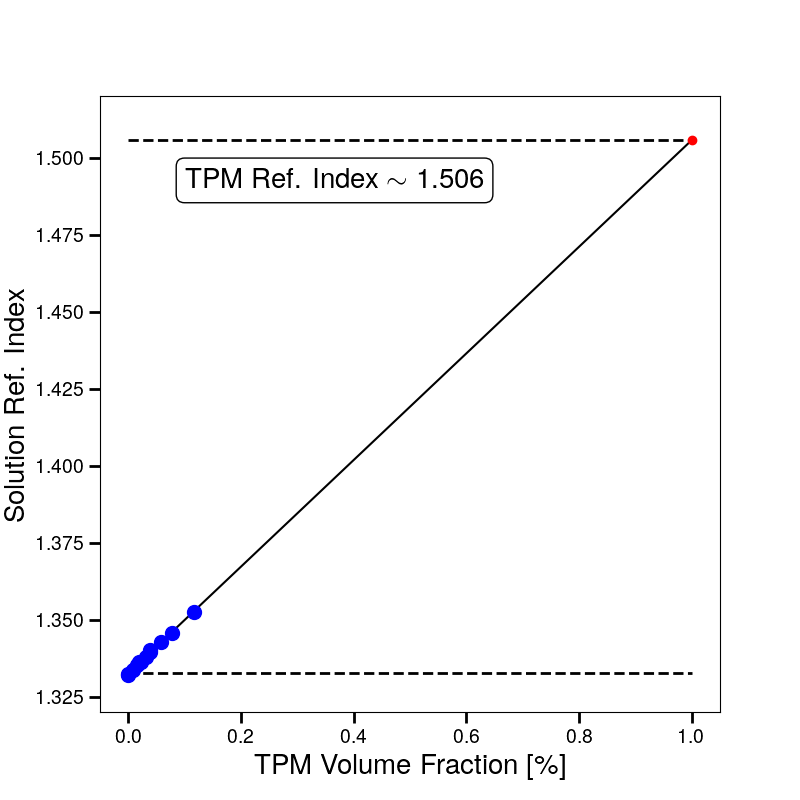
\includegraphics[width=0.7\columnwidth]{abbe_madness}
    \caption{Scatter plot of the measured refractive index of \num{12} solutions
      with differing volume fractions of TPM; each measurement is plotted as a filled
      blue circle.
      A linear fit to the data, represented as a solid black line, provides an estimate of
      the refractive index of polymerized TPM, $n_{\text{p}}$, represented as a red dot.
      The light blue region encompassing the linear fit denotes a $\SI{95}{\percent}$
      prediction interval that bounds the error in our extrapolated estimate of refractive
      index.
      The lower dashed line represents the refractive index of water at \SI{532}{\nm}.}
    \label{fig:abbe}
\end{figure}

%In general, there exists a linear relationship between the volume fraction of colloidal
%spheres, $\phi$, and the suspension refractive index. We estimate the refractive
%index of polymerized TPM spheres by extrapolating from our low volume fraction data
%up to a volume fraction of \num{1}. Our estimate is bounded by a $\SI{95}{\percent}$
%prediction interval given by
%\begin{align}
%  \text{Prediction Interval} &= \hat{n_{\text{p}}} \pm t_{\alpha/2, N-2} \, \sqrt{ S^2 +  S_{\hat{n_{\text{p}}}}^2} \\
%  S_{\hat{n_{\text{p}}}}^2 &= S^2 \, \left ( \frac{1}{N} + \frac{\left ( \phi^* - \bar{\phi_i} \right )}{Y} \right )\\ 
%  S^2 &= \frac{\sum_i \left (n_i - (m \, \phi + b )\right )^2}{N-1}\\
%  S_{\phi\phi} &= \sum_i \phi_i^2 - \left ( \sum_i \phi_i \right )^2 /N
%\end{align}

\begin{figure}
    \centering
    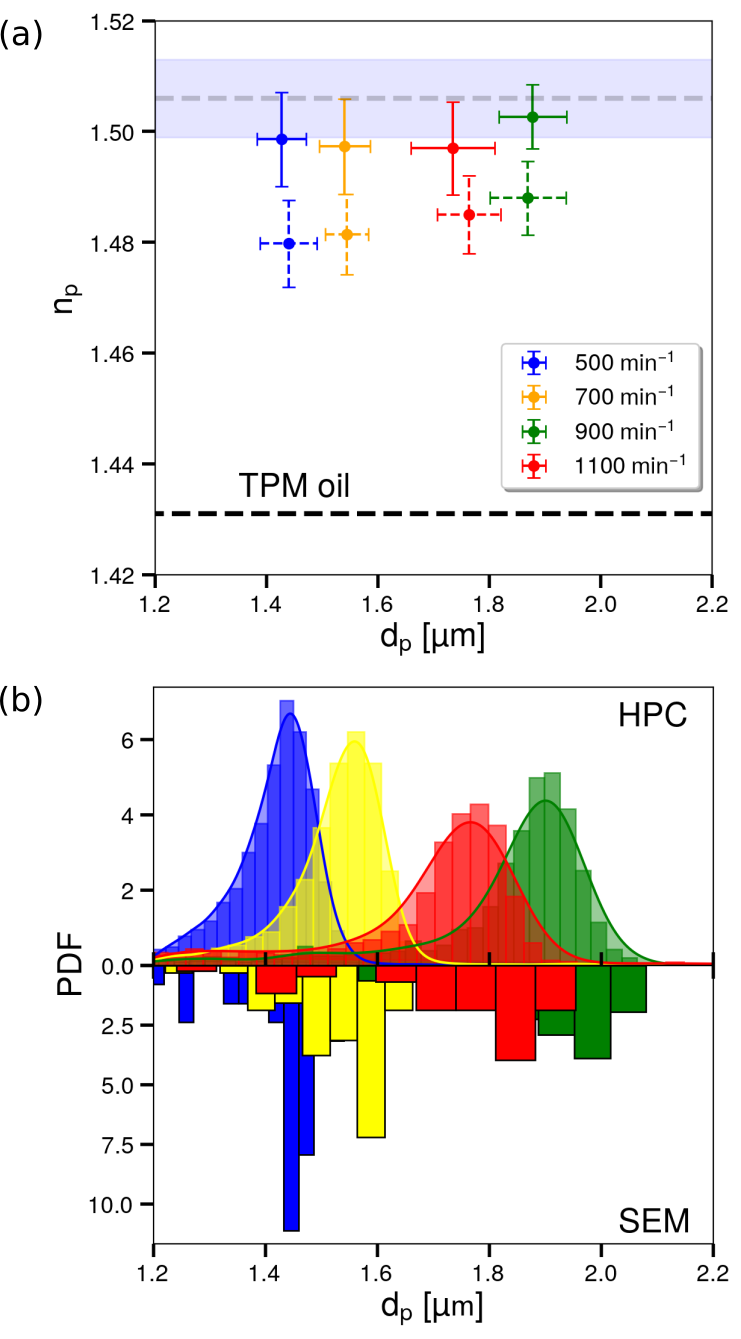
\includegraphics[width=0.5\columnwidth]{orthogonal_vs_hpc}
    \caption{(a) The result of HPC analysis for the unpolymerized (solid lines) and polymerized
      emulsions (dashed lines) stirred at \num{4} different stir rates. Filled circles
      represents the average diameter and refractive index and the associated error bars
      are set by a single median absolute deviation with the associated property.
      A dashed black line and a dashed grey line provide reference to the
      refractive index of monomeric TPM oil and our earlier estimate for TPM. The blue region
      fills the \SI{95}{\percent} prediction interval for our TPM estimate.
      TPM's refractive index. (b) Probability distributions of diameter as measured by
      HPC and by SEM analysis. HPC samples the diameter densely enough to allow
      reasonable kernel density estimation.}
    \label{fig:hpc_stir_rate}
\end{figure}


Results of holographic particle characterization for the four polymerized samples
and the four unpolymerized samples are summarized in Fig.~\ref{fig:hpc_stir_rate}(a).
Each dot represents the average size and refractive index for the associated sample.
Error bars are set by the single median absolute deviation of the associated property.
The unpolymerized droplets, represented with dashed error bars, have a systematically
lower refractive index than the polymerized droplets, represented with solid error bars.
Our extrapolated estimate of the refractive index is provided as a dashed gray
line with light blue region outlining a \SI{95}{\percent} prediction interval.

Holographic measurements report that the average refractive index of the
polymerized droplets
is $n_{\text{p}}=\SI{1.501(9)}{}$, which lies just within the prediction interval of our
previous measurement. The unpolymerized droplets have a systematically lower
refractive index.
Polymerization changes the chemical makeup of the droplet and generally increases the
density; %% FIXME: Add citation.
both processes might reasonably account for the observed change in refractive index.
The refractive indexes of TPM droplets and polymerized spheres both
substantially exceed that of bulk TPM oil, which is indicated by
a dashed line in Fig.~\ref{fig:hpc_stir_rate}(a).
Hydrolysis and oligomerization account for a refractive
index shift of roughly \SI{0.05} and polymerization accounts for the remaining
\SI{0.02} increase.

Fig.~\ref{fig:hpc_stir_rate}(b) summarizes measurements for the diameter, $d_{\text{p}}$,
obtained with holography and compares that with the distribution obtained
by SEM image analysis.
%The range of diameters is set to
%match the range set in Fig.~\ref{fig:hpc_stir_rate}(a), however, a small fraction of the data
%exist below $\SI{1.2}{\um}$.
Each holographic assay incorporates more than \num{3000} particle measurements.
The distribution of diameters is sampled densely enough to justify a kernel density
estimate of each population; the resulting kernel density estimates
are depicted in Fig.~\ref{fig:hpc_stir_rate}(b).
The average diameter increases with stir
rate from $\SI{500}{\minute^{-1}}$ to $\SI{900}{\minute^{-1}}$ but then decreases
at \SI{1100}{\minute^{-1}}. As the polydispersity greatly increases between
\SI{900}{\minute^{-1}} to \SI{1100}{\minute^{-1}}, we propose that the stir rate within
our vial induces shearing forces great enough to break up larger droplets.

SEM analysis confirms the results of holographic characterization for
particle sizes. All four distributions are
skew-left and their skewness increases with stir rate. The largest and smallest
observed diameters in each sample also coincide. The mean and median diameters
obtained holographically are systematically larger by a factor of $\SI{2}{\percent}$
than the results obtained by SEM. Presumably this difference can be explained
by shrinkage during SEM sample preparation \cite{yamada85,jung02}.

The principle difference between these measurements is that the holographic
results were obtained in a few minutes \emph{in situ} whereas both of
our orthogonal measurements require considerable sample preparation and
extensive data analysis.

% Abbe refractometry also takes more time and effort than holographic
% %%FIXME: Add David's edit?

\subsection{Monitoring polymerization}

We use heat-activated free radical initiators to polymerize TPM droplets.
Time-resolved holographic characterization can monitor the progress of
this process starting with the addition of initiator.
As observed in Fig.~\ref{fig:hpc_stir_rate}(a), the polymerization of
liquid TPM droplets induces an increase of \SI{0.02}{} in refractive index,
which is well within the resolution of the xSight.  Because the refractive index
of a material is a function of its composition \cite{wang15},
refractive index serves as a proxy for the degree of polymerization.
Holographic particle characterization is uniquely poised to probe the time dependent
polymerization of TPM as it can monitor the refractive index of individual spheres
\emph{in situ}.

We investigate the polymerization rate of TPM droplets by regularly sampling a
suspension undergoing polymerization and characterizing each drawn sample with HPC.
Specifically, the suspension consists of an emulsion of TPM droplets
and the initiator AIBN. The suspension is continuously stirred at \SI{1100}{\min^{-1}}
and is thermally coupled to a heat bath set at \SI{80}{\degreeCelsius}.
We draw \SI{1}{\ul} of the suspension after \num{0}, \num{5}, \num{10}, \num{15},
\num{20}, \num{40}, \SI{60}{\min}, and \SI{120}{\min} as the sample undergoes polymerization.
Each sample was added to \SI{10}{\milli\liter} of room temperature deionized water,
which effectively arrests polymerization. 
Each sample is then immediately characterized by the xSight.

\begin{figure}
    \centering
    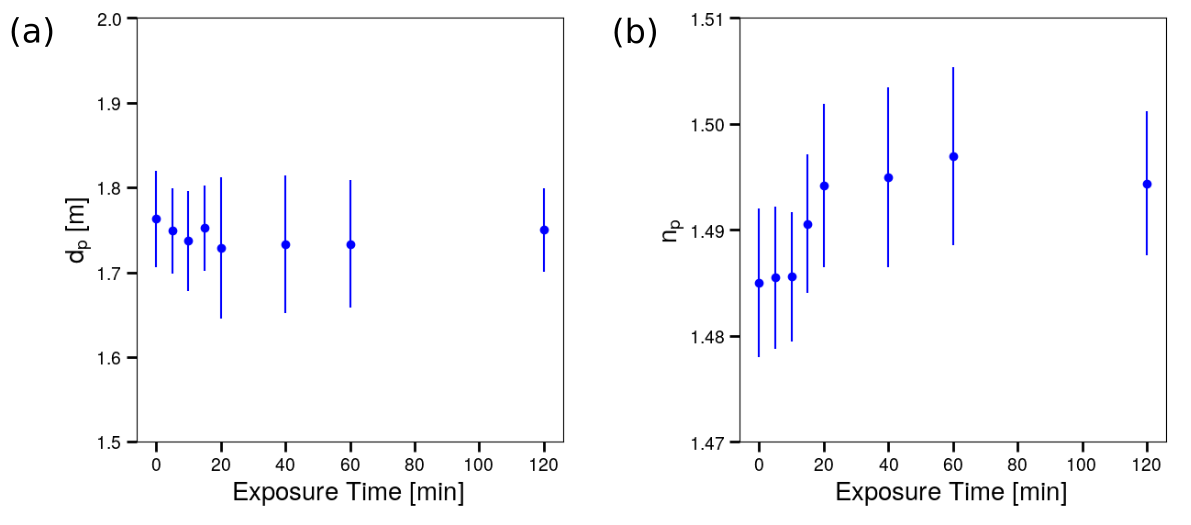
\includegraphics[width=\columnwidth]{synthesis_heat_bath}
    \caption{Particle properties after heat bath exposure times of \num{0}, \num{5},
      \num{10}, \num{15}, \num{20}, \num{40}, \SI{60}{\min}, and \SI{120}{\min}.
      (a) The average size and (b) refractive index of particles as a function
      of heat bath exposure time. Error bars indicate a single median absolute deviation
      of the associated property.}
    \label{fig:heat_size_time}
\end{figure}

Figure ~\ref{fig:heat_size_time} depicts the result of this series of
measurements. The diameter of the TPM droplets shrink by \SI{2}{\percent} on average
during polymerization.
Although this is well within the
measured polydispersity of each sample, it is consistent with the \SI{7}{\percent} reduction
in volume reported in Ref.~\cite{vanderwel17}. % FIXME: reported may be overstating.
Fig.~\ref{fig:heat_size_time}(b) demonstrates a simultaneous large shift in refractive index
from \SI{1.485}{} for unpolymerized droplets to \SI{1.495}{} for the droplets
exposed to the heat bath for two hours. The increase in refractive index occurs almost
entirely in \SI{20}{\minute} of exposure to \SI{80}{\degreeCelsius}.
Van der Wel \emph{et al.} \cite{vanderwel17} suggest heating the suspension
for \SI{2}{\hour} to ensure the sample has sufficiently polymerized and is
stable. Our analysis suggests heating for \SI{20}{\minute} will produce
particles with similar properties. %, although continued polymerization may yield more stable particles.
Because holographic characterization can be performed in a matter of minutes,
this information can be used to monitor polymerization and to stop processing
once it has run to completion. This information can minimize heating time
and thus energy cost in colloidal polymerization.

\subsection{Effect of emulsion stoichiometry and choice of free radical initiator}

Increasing the amount of TPM oil available in solution could increase the
average particle diameter, the number of resulting colloidal particles, or both.
In addition, increasing the pH of the solution will increase the rate of
oligomerization and could affect the average particle diameter and polydispersity.
To probe these two influences on droplet formation, we prepare four batches of droplets
corresponding to binary choices in concentrations of TPM oil and ammonium chloride
added to \SI{5}{\milli\liter} of deionized water.
Batches A and B contain
\SI{100}{\micro\liter} of TPM with \si{10} and \SI{20}{\micro\liter} of 
ammonia added, respectively. Batches C and D contain \SI{150}{\micro\liter} of TPM oil, 
again with \si{10} and \SI{20}{\micro\liter} of ammonia, respectively.

% FIXME: We do not have results (?) for the unpolymerized droplets from
% batches A, B, C, or D in May 2018. We do have some results from Jan 2018
% but that is from a different synthesis. :-/
%\SI{0.1}{\percent} sodium docecyl sulfate (SDS) was introduced to
%each sample to suppress aggregation. Through this, we can observe the effects of
%varying the amount of TPM and the pH on the size of the resulting droplets.

% XXX (Add conclusions about initiator- does not seem to matter)

To investigate the choice of free radical initiator, we polymerized each of the four
above emulsions with four different initiators:
two water-insoluble initiators, AIBN and
\num{1},\num{1}'-azobis(cyclohexanecarbonitrile) (ACHN, Sigma Aldrich),
and two water-soluble  initiators, potassium persulfate (KPS, Sigma Aldrich) and
ammonium persulfate (APS, Sigma Aldrich).
Each of the four stoichiometric assays were polymerized with each of the four
radical initiators to make a total of \num{16} samples.
Specifically, for each of the four stoichiometric assays, four \SI{1}{\milli\liter} of
samples of emulsion droplets are prepared in \SI{1.5}{\milli\liter} microcentrifuge tubes.
Each \SI{1}{\milli\liter} sample is individually combined with \SI{1}{\milli\gram} of
a specific initiator.
All sixteen samples are then polymerized at \SI{80}{\celsius} for \SI{12}{\hour}
on a shaker set at \SI{750}{\minute^{-1}}. Continuous agitation is intended to
maintain well-mixed reaction conditions, with the goal of reproducibly creating
monodisperse samples.
The resulting polymerized spheres are then individually analyzed with the xSight.

\begin{figure}
    \centering
    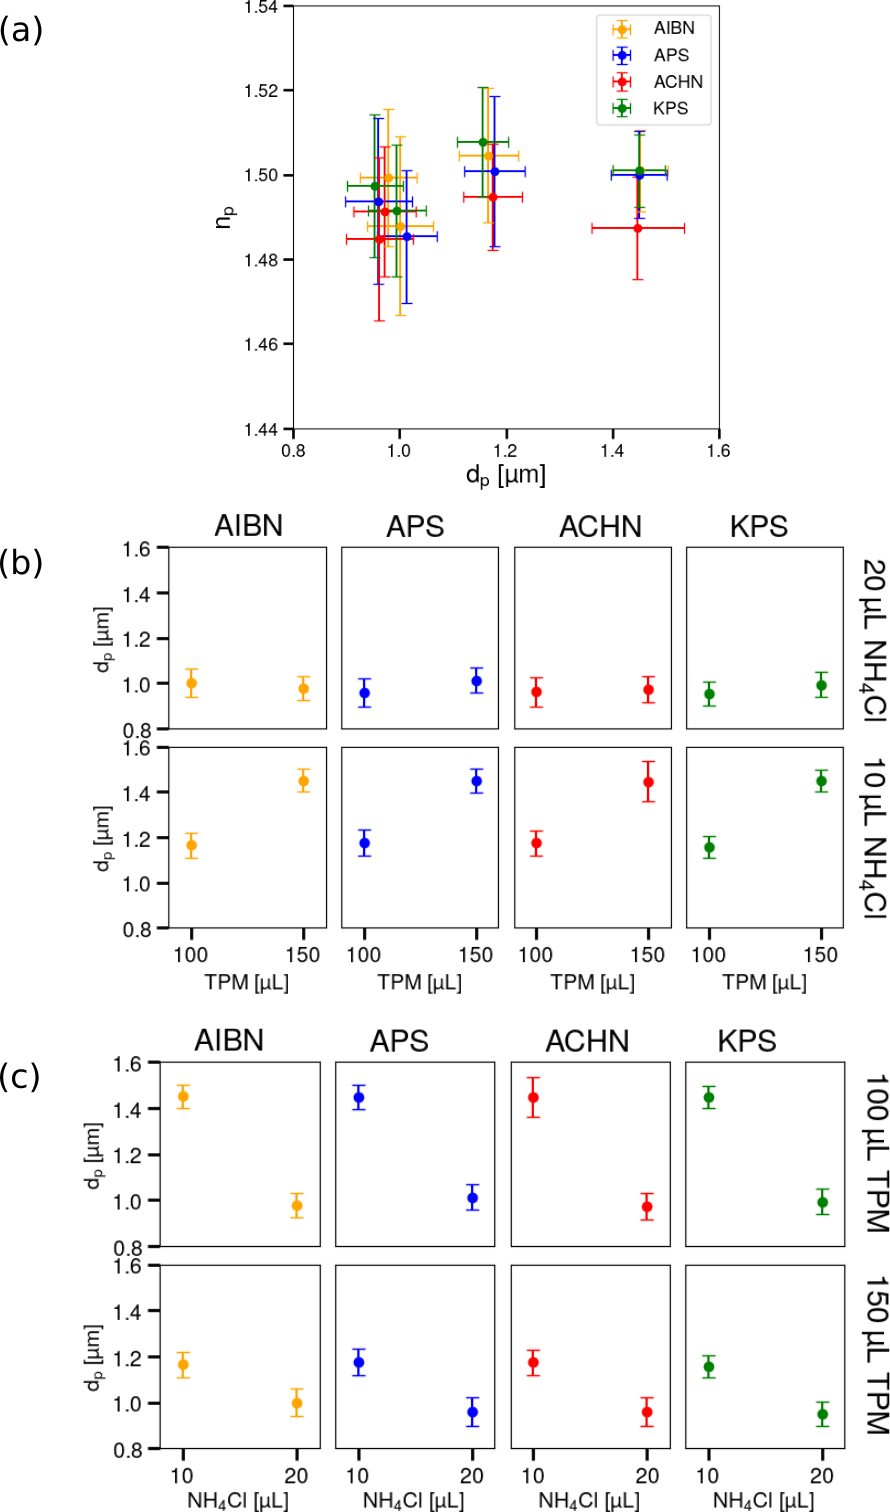
\includegraphics[width=0.7\columnwidth]{longitudinal_summary.png}
    \caption{Holographic characterization results for various initiators and
      emulsion compositions. (a) The average refractive index and diameter of
      all \num{16} samples of polymerized TPM spheres.
     (b) Mean diameter as a function of TPM added at fixed ammonium chloride.
     (c) Mean diameter as a function of ammonium chloride added at fixed TPM.}
    \label{fig:longitudinal_summary}
\end{figure}

Fig.~\ref{fig:longitudinal_summary}(a) shows the results from all \num{16} data sets.
The average diameter and refractive index of a few thousand particles from each sample
are presented as points with error bars extending to one median absolute deviation
of the associated parameter. Clusters of points are associated with particular
stoichiometries, the largest being formed with higher TPM concentration
and lower ammonium chloride concentration.
To identify trends, we unpack the two dependent variables from the three
parameters we varied and present the  results for particle size in
Fig.~\ref{fig:longitudinal_summary}(b) and (c).

Fig.~\ref{fig:longitudinal_summary}(b) fixes the initiator choice and the
amount of ammonium chloride added to isolate the influence of TPM concentration
on the resulting average particle diameter. Qualitatively, we can see that
choice of initiator had little to no effect in determining the finished particle's
average diameter. In the first row, each of the four assays has \SI{10}{\micro\liter}
of ammonium chloride added; in this regime, adding more TPM oil
creates larger particles. In the second row, each of the four
assays has \SI{20}{\micro\liter} of ammonium chloride added; in this regime, adding
more TPM oil has little to no effect in determining the average particle diameter.

Fig.~\ref{fig:longitudinal_summary}(c) shows the complementary projection
of the data by fixing the amount of TPM added to isolate the influence of
ammonium chloride concentration. All eight assays convey the same message:
an increase in ammonium chloride concentration results in a decrease in
average particle diameter.

The result of this assays tells a compelling story. The choice of initiator plays little
to no role in determining average particle size. This is sensible as the emulsification
of TPM oil determines the droplet size and polymerization is thought to only
shrink the particle. The concentration of ammonium chloride increases the pH and
therefore increases the rate at which TPM hydrolizes and oligomerizes. Faster nucleation
yields more droplets and reduces the average particle size.
At low concentrations of ammonium chloride, the oligomerization process is slower
and yields fewer droplets; more TPM oil in this context provides more oligomerized
TPM to grow droplets. At high concentrations of ammonium chloride, the oligomerization
process occurs quickly and yield many droplets; more TPM oil in this context produces
more droplets.


\begin{figure}
    \centering
    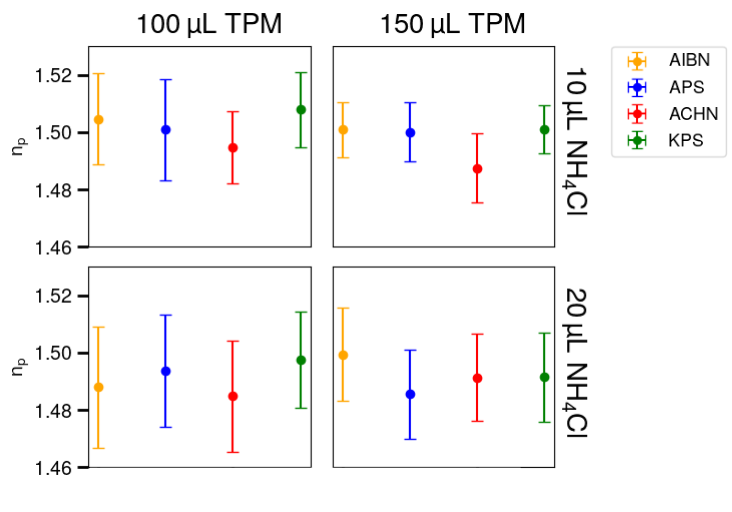
\includegraphics[width=0.75\columnwidth]{longitudinal_np.png}
    \caption{Mean refractive index reported for each radical initiator
    at fixed TPM}
    \label{fig:longitudinal_np}
\end{figure}

The results presented in Fig.~\ref{fig:longitudinal_summary}(a) also provide information
on the average refractive index of polymerized TPM spheres. Although polymerization
has little effect on the distribution of particle diameters, we already have seen that
polymerization induces a sizable change in refractive index. Fig.~\ref{fig:longitudinal_np} therefore isolates the
variables of droplet formation, namely the amount of TPM and ammonium chloride added,
and isolates the influence of initiator choice on the average refractive index.

%% FIXME: Consider David's edit

Interestingly, holographic characterization reveals no discernible difference
in the particles' refractive indexes.
Under certain conditions, TPM droplets are known to form dimpled spheres when polymerized
with the water-soluble initiators APS and KPS due to the ejection of low molecular weight
oligomers \cite{sacanna11}.
Therefore, one might think that TPM spheres polymerized with these initiators would be
made of on average higher molecular weight oligomers and have a higher refractive index
than pa. However, under the conditions observed here where no dimple was formed, there
was no observable difference in particle size or refractive index between the initiators
used.

\section{Discussion}

We have demonstrated the use of holographic particle characterization
to investigate the emulsion polymerization of TPM. Our study examines the
role certain synthesis protocols play in determining the
size and refractive index of the resulting polymerized spheres. Specifically,
we investigate the role of stir rate, the time spent heat-activated, stoichiometry, and choice of
free radical initiator.

The polydispersity in particle diameter was found to increase
with stir rate. While an initial increase with particle diameter is observed with increasing
stir rate, we believe the increase in polydispersity confounds this trend.
Unlike the orthogonal techniques we used to support our analysis,
holography can provide immediate feedback on the size and refractive index of unpolymerized
droplets. By periodically sampling the distribution of sizes and refractive indexes of
droplets undergoing polymerization, we determined that changes in the optical properties
of TPM spheres mostly occur in the first \SI{20}{\minute}. Finally, we observed
influence of emulsion stoichiometry and free radical initiator.
With our particular synthesis, we isolated a complex
relationship between the pH of the solution and the amount of TPM added
during emulsification: at low pH, increases in TPM yield \emph{larger}
particles and at high pH, increases in TPM yield \emph{more} particles.

%We chose the synthesis of TPM as it is a model system for many colloidal studies, yet holography
%can be used to diagnose the relationship between environment conditions and
%particle properties for other syntheses. Future studies may employ concentration
%measurements to better resolve the complex relationship between the many existing
%synthesis parameters.

These results demonstrate that holographic characterization can be a valuable
addition to the arsenal of techniques used to design and control colloidal
synthesis.

\section{Acknowledgment}

This work was supported primarily by the MRSEC program of
the National Science Foundation through Award Number DMR-1420073.
Additional support was provided by the SBIR program of the
National Science Foundation through Award Number IPP-1519057.
The FESEM was purchased with financial support from the MRI program
of the National Science Foundation under Award DMR-0923251.
